% Important: If latex complains about unicode characters,
% please use "\usepackage[utf8x]{inputenc}" in your preamble
% You can change the size of the picture by putting it into the construct:
% 1) \resizebox{10cm}{!}{"below picture"} to scale horizontally to 10 cm
% 2) \resizebox{!}{15cm}{"below picture"} to scale vertically to 15 cm
% 3) \resizebox{10cm}{15cm}{"below picture"} a combination of above two
% It is not recomended to use the scale option of the tikzpicture environment.
\resizebox{10cm}{!}{
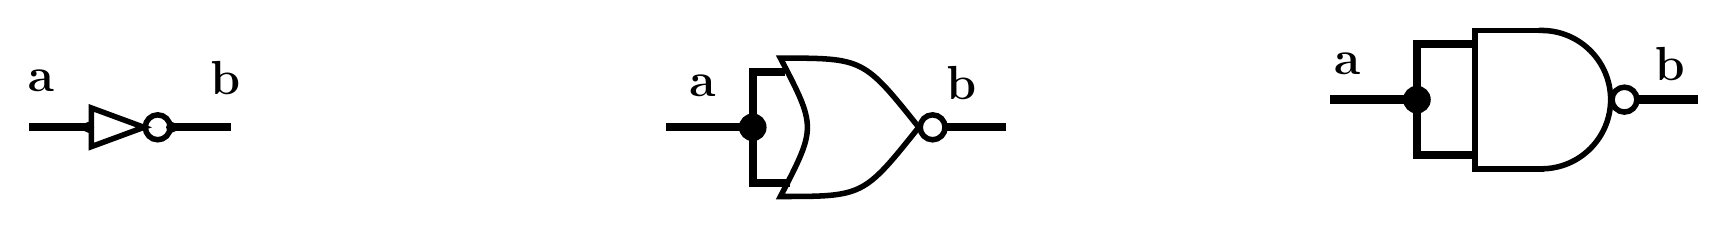
\begin{tikzpicture}[x=1pt,y=-1pt,line cap=rect]
\def\logisimfontA#1{\fontfamily{cmr}{#1}} % Replaced by logisim, original font was "SansSerif"
\definecolor{custcol_0_0_0}{RGB}{0, 0, 0}
\definecolor{custcol_ff_ff_ff}{RGB}{255, 255, 255}
\draw [line width=3.0pt, custcol_0_0_0 ]  (531.0,11.0) -- (511.0,11.0) -- (511.0,31.0) -- (511.0,51.0) -- (531.0,51.0) ;
\draw [line width=3.0pt, custcol_0_0_0 ]  (591.0,31.0) -- (611.0,31.0) ;
\draw [line width=3.0pt, custcol_0_0_0 ]  (241.0,41.0) -- (271.0,41.0) ;
\draw [line width=3.0pt, custcol_0_0_0 ]  (341.0,41.0) -- (361.0,41.0) ;
\draw [line width=3.0pt, custcol_0_0_0 ]  (481.0,31.0) -- (511.0,31.0) ;
\draw [line width=3.0pt, custcol_0_0_0 ]  (11.0,41.0) -- (31.0,41.0) ;
\draw [line width=3.0pt, custcol_0_0_0 ]  (61.0,41.0) -- (81.0,41.0) ;
\fill [line width=3.0pt, custcol_0_0_0]  (271.0,41.0) ellipse (5.0 and 5.0 );
\fill [line width=3.0pt, custcol_0_0_0]  (511.0,31.0) ellipse (5.0 and 5.0 );
\draw [line width=2.0pt, custcol_0_0_0 ]  (51.0,41.0) -- (32.0,34.0) -- (32.0,48.0) -- cycle;
\draw [line width=2.0pt, custcol_0_0_0]  (56.0,41.0) ellipse (4.5 and 4.5 );
\fill [line width=2.0pt, custcol_0_0_0]  (61.0,41.0) ellipse (2.0 and 2.0 );
\fill [line width=2.0pt, custcol_0_0_0]  (31.0,41.0) ellipse (2.0 and 2.0 );
\logisimfontA{\fontsize{16pt}{16pt}\fontseries{bx}\selectfont\node[inner sep=0, outer sep=0, custcol_0_0_0, anchor=base west] at  (75.0,29.0)  {b};}
\logisimfontA{\fontsize{16pt}{16pt}\fontseries{bx}\selectfont\node[inner sep=0, outer sep=0, custcol_0_0_0, anchor=base west] at  (597.0,24.0)  {b};}
\logisimfontA{\fontsize{16pt}{16pt}\fontseries{bx}\selectfont\node[inner sep=0, outer sep=0, custcol_0_0_0, anchor=base west] at  (341.0,31.0)  {b};}
\logisimfontA{\fontsize{16pt}{16pt}\fontseries{bx}\selectfont\node[inner sep=0, outer sep=0, custcol_0_0_0, anchor=base west] at  (248.0,30.0)  {a};}
\draw [line width=2.0pt, custcol_0_0_0] (556.0,56.0) arc (90.0:-90.0:25.0 and 25.0 );
\draw [line width=2.0pt, custcol_0_0_0 ]  (556.0,6.0) -- (532.0,6.0) -- (532.0,56.0) -- (556.0,56.0) ;
\draw [line width=2.0pt, custcol_0_0_0]  (586.0,31.0) ellipse (4.5 and 4.5 );
\logisimfontA{\fontsize{16pt}{16pt}\fontseries{bx}\selectfont\node[inner sep=0, outer sep=0, custcol_0_0_0, anchor=base west] at  (9.0,28.0)  {a};}
\logisimfontA{\fontsize{16pt}{16pt}\fontseries{bx}\selectfont\node[inner sep=0, outer sep=0, custcol_0_0_0, anchor=base west] at  (481.0,22.0)  {a};}
\draw [line width=3.0pt, custcol_0_0_0 ]  (281.0,21.0) -- (281.0,21.0) -- (271.0,21.0) -- (271.0,41.0) -- (271.0,61.0) -- (281.0,61.0) -- (283.0,61.0) ;
\draw [line width=2.0pt, custcol_0_0_0 ]  (331.0,41.0) .. controls  (311.0,16.0)  ..  (281.0,16.0) .. controls  (294.0,41.0)  ..  (281.0,66.0) .. controls  (311.0,66.0)  ..  (331.0,41.0) -- cycle ;
\draw [line width=2.0pt, custcol_0_0_0]  (336.0,41.0) ellipse (4.5 and 4.5 );
\end{tikzpicture}
}
